\section{Proposal}
\label{sec:Proposal}

This Section wraps up the previous considerations by making a partial proposal
for the missing elements, so that it becomes possible to demonstrate that our vision
works. We demonstrate that it becomes possible to specify MAs independently of the
MT specifying a \DSL's execution semantics; that several MAs may be linked to
the same MT for animating a model according to the viewer's preferences; and finally
that MAs may be reused accross \DSLs.

%We start by specifying a prototype metamodel \textsf{CS} for specifying concrete
%syntaxes explicitly. We then define 

\subsection{\textsf{VCS}: A Visual Concrete Syntax \DSL}
\label{sec:Proposal-VCS}

\autoref{fig:VCS} shows the metamodel of \textsf{VCS}, a simplified \DSL designed
for the specification of Visual Concrete Syntaxes. It consists of a \textsf{Canva}
of variable size where graphical elments (\textsf{GElement}) may be geometrically
placed. A \textsf{GElement} follows the Composite Pattern \citep{B:Gamma-etAl:1995}:
\textsf{Shape}s may be \emph{composed}, i.e. the \textsf{containee} is displayed
\emph{inside} the \textsf{container} with specific alignment features. 

A \textsf{Shape} is either a \textsf{Table}, a \textsf{TextBox}, or a 
\textsf{Geometric} element, which is either a \textsf{Form} or a 
\textsf{Connector}. Each \textsf{Shape} is inscribed into a bounding box with specific 
dimensions that helps precisely positioning it on the \textsf{Canva}, and also
defines specific features: for example, a Rectangle may define the thickness of its
external box, and an Arrow may define different types and sizes for their heads.
A \textsf{Shape} may also define a \textsf{Style} that can be \textsf{name}d and
reused across other \textsf{Shape}s, to specify various features such as the background
or line colour, the line transparency, etc.

This metamodel captures insideness with \textsf{Composer}, and may easily be extended
with additional \textsf{Shape}s that only need to be encapsulated in a box (thus,
giving value to the attributes \textsf{length} and \textsf{height} in \textsf{Shape}).


\begin{figure}[t]%
   \centering
   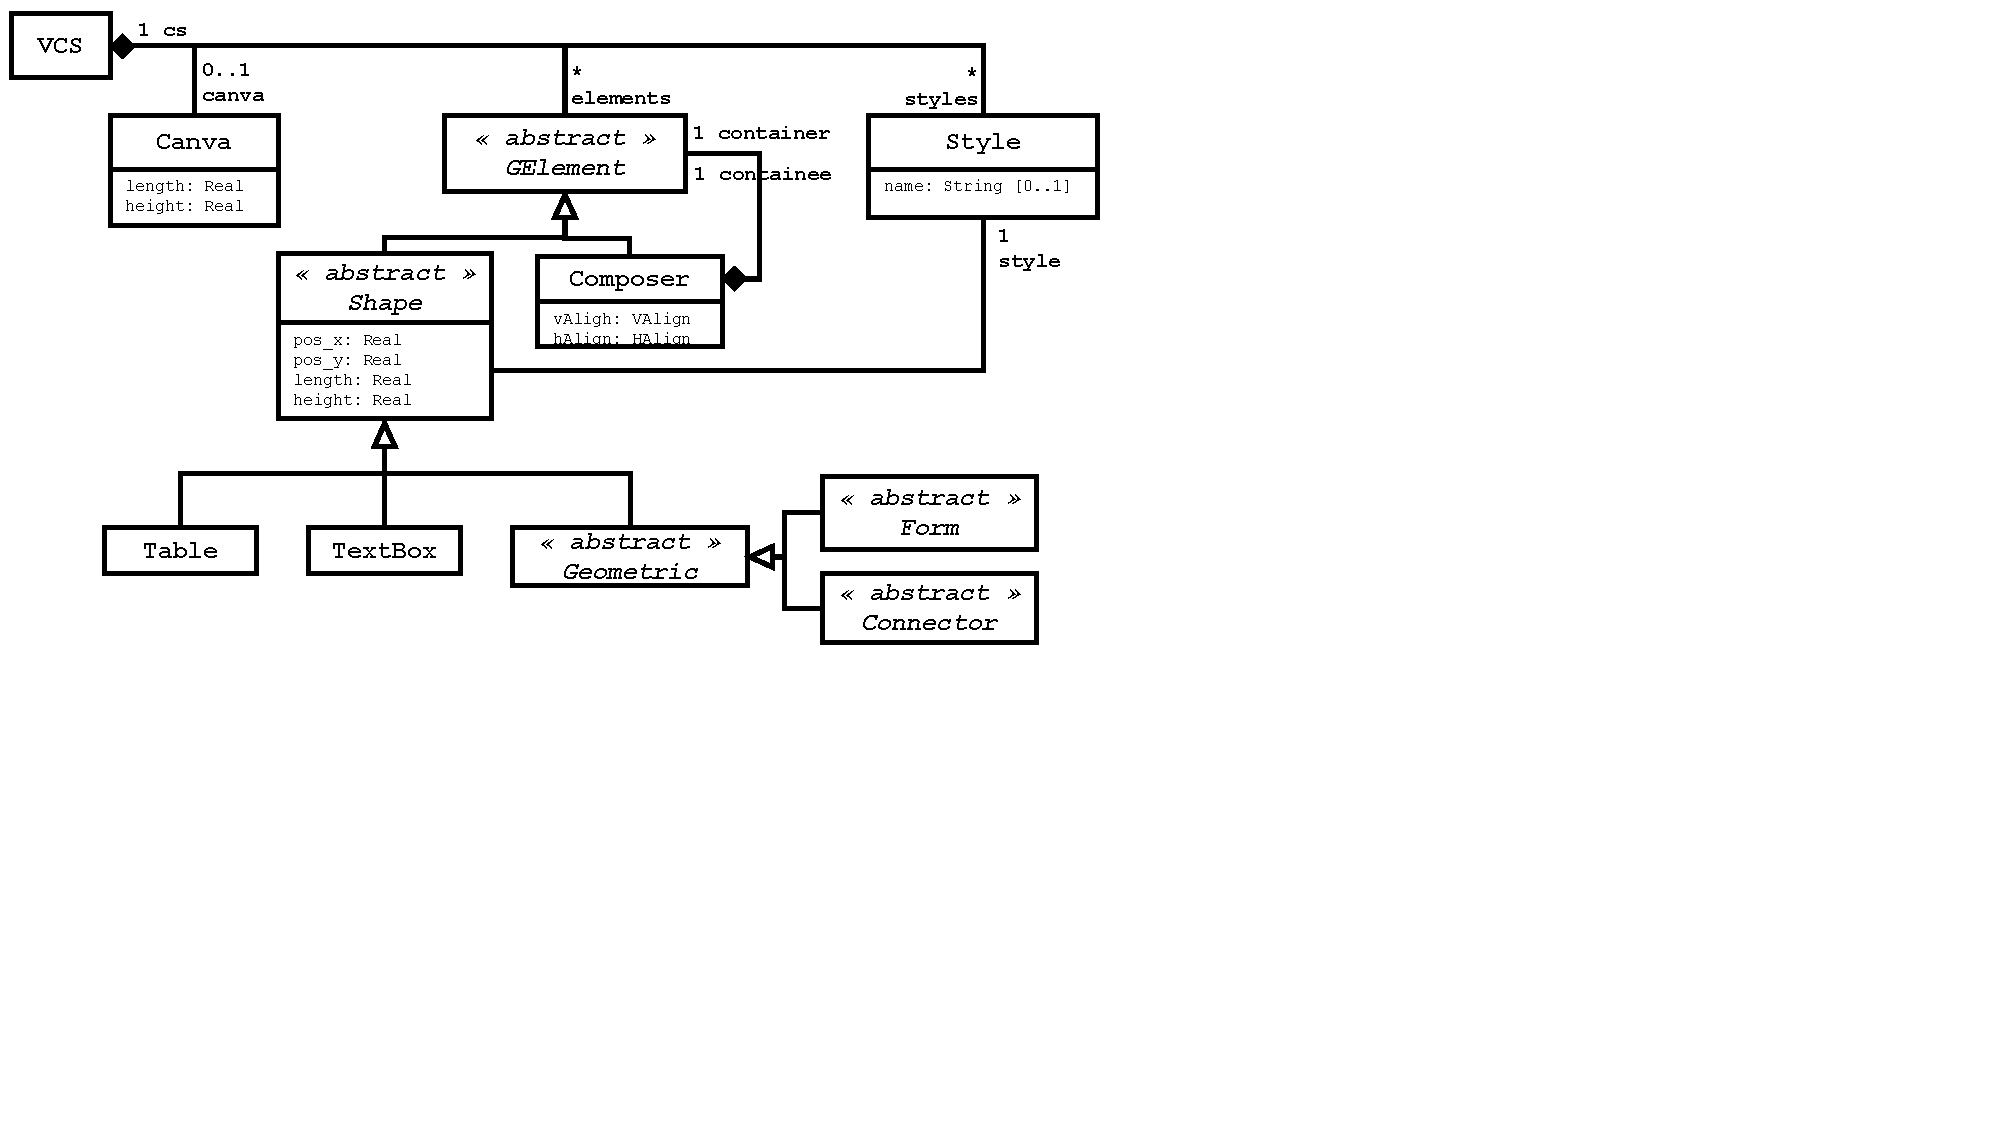
\includegraphics[width=\columnwidth,clip, trim=0cm 8cm 15cm 0.2cm]{VCS}%
   \caption{\textsf{VCS}: A simplified \DSL for specifying \emph{V}isual \emph{C}oncrete \emph{S}yntaxes}%
   \label{fig:VCS}%
\end{figure}


\subsection{Revisiting the \textsf{FSM}}
\label{sec:Proposal-FSM}



\subsubsection{Concrete Syntax}
\label{sec:Proposal-FSM-CS}


The first step is to define a mapping from the \textsf{FSM} metamodel (cf. \autoref{fig:FSM_MM})
to (a model of) \textsf{VCS}. Since defining the mapping rigorously requires the
definition of a specific \DSL, we rely on the reader's intuition and explain 
informally how it is done.

Following the traditional approach in \MDE, defining a mapping results in an 
(semi-)automatically generated so-called \emph{palette} presenting to a modeller
the visual components that can be used for creating, and editing models. The palette
in itself is not difficult to create from the mapping, but to obtain a fully-fledged
syntax-oriented editor, additional constraints for well-formedness need to be added,
which is out of our scope for now. Furthermore, editing flexibility for some visual
components is required to ease model creation: typically, any kind of arrow, eventually
supported by routing algorithms, may be at disposal of the modeller instead of forcing
one kind of arrow for any diagram.

The \textsf{FSM} class is mapped to the overall diagram supported by the \textsf{Canva},
accompanied with a \textsf{TextBox} that will display \textsf{FSM::name}.
A (\textsf{REGULAR}) \textsf{State} is represented by an \textsf{Ellipse} with equal \textsf{length}
and \textsf{height} (thus creating a circle) drawn in plain black. A \textsf{FINAL}
one is mapped to a \textsf{Composite}: two \textsf{Ellipse}s vertically and horizontally
centered, with \textsf{length} and \textsf{height} only differing by the same delta.
An \textsf{INITIAL} \textsf{State} will be represented similar to a \textsf{REGULAR}
one, except it will be drawn in dotted red to distinguish it. This allows us to not
bother with aligning an arrow into an \textsf{Ellipse} for now. Finally, a 
\textsf{Transition} may be mapped to any instance of an \textsf{Connector} drawn
in black, plain line with the same thickness as the \textsf{State}'s \textsf{Ellipse}s,
assuming they present an \textsf{ArrowHead} with a specific size and type. Finally,
\textsf{Token} is mapped to a plain red \textsf{Ellipse} with dimensions the fourth
of the ones used for \textsf{State}, and are systematically placed at the horizontal
and vertical center of the \textsf{State}'s \textsf{Ellipse} it \textsf{current}ly
points to.

\subsubsection{Selected Animations}
\label{sec:Proposal-FSM-ANIM}

The second step is to define, and attach, animations (units) to Transformation 
Units. We will consider two versions of the transformation \textsf{accept(word :
Word)}, which iteratively calls a TU \textsf{fire} that performs the firing, 
until the \textsf{word} is empty (in which case, it remains to check whether 
the current \textsf{State} is \textsf{FINAL}), or no \textsf{Transition} is 
fireable (i.e. \textsf{fire} does not return anything, in which case the 
\textsf{word} is rejected).
\begin{enumerate}
	\item The \textsf{fire} TU simply loops over all possible outgoing \textsf{Transition}
   to find one that is fireable, i.e. whose \textsf{trigger} matches the current \textsf{Letter}.
   
   \item The \textsf{fire} TU performs the same algorithm, except that it calls
   another TU \textsf{getEnabledTransition} that returns one (of the possible) matching
   \textsf{TRansition}(s).
\end{enumerate}

\begin{figure}[t]%
   \centering
   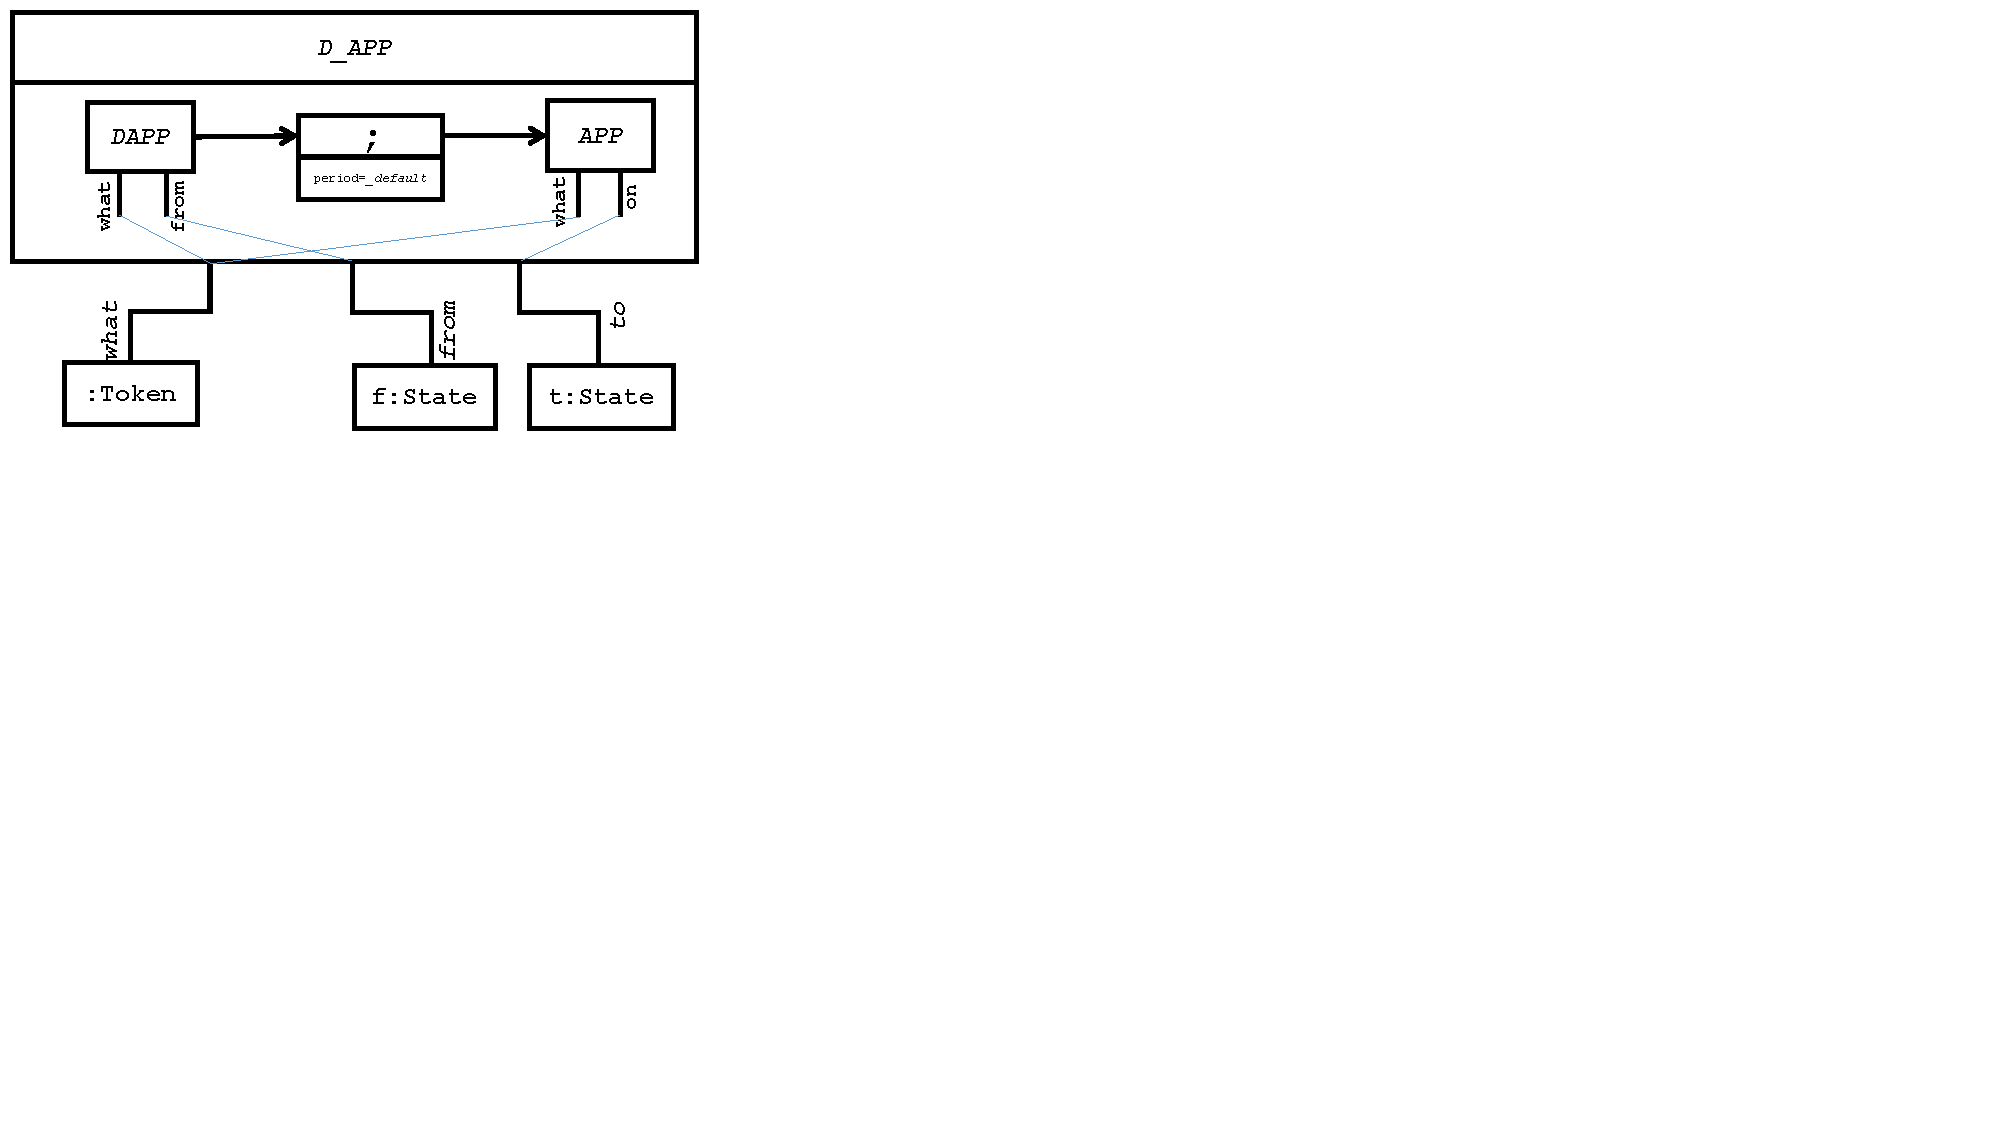
\includegraphics[width=\columnwidth,clip, trim=0cm 11.5cm 22cm 0.2cm]{D_APP}%
   \caption{\textsf{VCS}: A simplified \DSL for specifying \emph{V}isual \emph{C}oncrete \emph{S}yntaxes}%
   \label{fig:VCS}%
\end{figure}

We now define AUs for these two transformations. The animation \textsf{D\_APP}
implements \textsf{FSM.2.1}: it makes the \textsf{Token}'s \textsf{Ellipse} 
disappear from the current \textsf{State} (named \textsf{f}), then reappear 
into the target one (named \textsf{t}). 
The animation \textsf{BLINK} (in \autoref{fig:UA-Param})implements \textsf{FSM.2.3}:
it makes the \textsf{Transition}'s \textsf{Connector} blink for 3 seconds.
With these definitions, we can proceed to the mapping between TUs and AUs:

$$\begin{array}[t]{l}
   \textbf{Transformation (1)}\\
   \mathsf{fire} \mapsto \mathsf{D\_APP}
\end{array}
\hspace{0.5cm}
\begin{array}[t]{lcr}
   \multicolumn{2}{c}{\textbf{Transformation (2)}}\\
	\mathsf{fire} &\mapsto& \mathsf{D\_APP}\\
	\mathsf{getEnabledTransition} &\mapsto& \mathsf{BLINK}	
\end{array}$$

Note that in this case, we chose to use models' elements: in order to appropriately
identify them, the annotations on the TUs may explicitly indicate them, and even
map them to the UAs' parameters. 

\subsubsection{Reusing AUs}
\label{sec:Proposal-Reuse}

\textsf{D\_APP} could be reused for \textsf{PM.1}, with \textsf{:PacMan},
\textsf{:Cell} and \textsf{:Cell} as parameters, and for \textsf{PN.3.1}
with \textsf{markings}, \textsf{:Place} and \textsf{:Place}. Similarly,
\textsf{BLINK} could be reused for \textsf{PN.2} with \textsf{:Transition}
and a predefined \textsf{period}. Note that all these UAs should be
effectively linked to the respective TUs of the \DSLs to fully work.
